\chapter{Dynamic Programming}

\begin{important}[Paradigm]
Dynamic programming (DP) solves a problem by combining solutions to \textbf{overlapping subproblems},
each solved once and stored in a table. It applies when the problem has \textbf{optimal substructure}:
an optimal solution is built from optimal solutions to subproblems.
\end{important}

\paragraph{Recipe.}
\begin{enumerate}
  \item Define the subproblems precisely (``$M[i]$ = the optimal value for \dots'').
  \item Write a recurrence for $M[i]$ in terms of smaller subproblems, with base cases. Justify it: consider what an
        optimal solution does with the last element/choice.
  \item Choose an evaluation order so that dependencies are computed first (bottom-up), or memoize (top-down).
  \item Runtime $=$ (number of subproblems) $\times$ (time per subproblem). Space is the table size.
  \item Recover the actual solution by tracing back through the table (store the choice made, or recompute it).
\end{enumerate}

\begin{example}[Why tables]
Naive recursion for $F(n)=F(n-1)+F(n-2)$ takes $\Theta(\varphi^n)$ because $F(n-k)$ is recomputed many times.
Filling $F[0..n]$ left to right takes $\Theta(n)$ additions.
\end{example}

\section{Weighted interval scheduling}
Intervals $i=1..n$ with weights $v_i$, sorted by finish time $f_1\le\dots\le f_n$. Find a compatible set of max total weight.
(Greedy fails once weights are present.) Let $p(j)$ be the largest index $i<j$ with $f_i\le s_j$ (0 if none).

Let $M[j]$ be the max weight using intervals $1..j$. An optimal solution either excludes $j$, or includes $j$ and then
only intervals $1..p(j)$ remain usable:
\[
M[0]=0,\qquad M[j]=\max\bigl(M[j-1],\;v_j+M[p(j)]\bigr).
\]
\begin{lstlisting}[style=pseudo]
sort by finish time; compute p(1..n) by binary search   // $\bigO(n \log n)$
M[0] = 0
for j = 1 to n do M[j] = max(M[j-1], $v_j$ + M[p(j)])
// traceback
j = n
while j > 0 do
    if $v_j$ + M[p(j)] >= M[j-1] then output j; j = p(j)
    else j = j - 1
\end{lstlisting}
Total $\Theta(n\log n)$; the DP itself is $\Theta(n)$.

\begin{figure}[H]
\centering
\begin{tikzpicture}[x=0.7cm, y=0.6cm, font=\small, >=Stealth]
  \foreach \j/\s/\f/\v/\p/\M in {1/0/3/2/0/2, 2/1/5/4/0/4, 3/4/6/4/1/6, 4/2/8/7/0/7, 5/6/9/2/3/8, 6/7/10/1/3/8} {
    \node[anchor=east, font=\scriptsize] at (-0.3,-\j) {$j=\j$, $v=\v$};
    \draw[line width=4pt, blue!40] (\s,-\j) -- (\f,-\j);
    \node[anchor=west, font=\scriptsize] at (10.8,-\j) {$p(j)=\p$};
    \node[anchor=west, font=\scriptsize] at (13.2,-\j) {$M[j]=\M$};
  }
  \draw[->, red!70!black, thick] (4,-3) to[out=150, in=-30] (3,-1);
  \draw[->, red!70!black, thick] (6,-5) to[out=150, in=-30] (6,-3);
  \draw[->, red!70!black, thick] (7,-6) to[out=150, in=-30] (6,-3.1);
  \draw[->] (0,-6.8) -- (10.4,-6.8);
  \foreach \x in {0,2,...,10} \draw (\x,-6.8) -- (\x,-7.0) node[below, font=\scriptsize]{\x};
\end{tikzpicture}
\caption{Six weighted intervals sorted by finish time. Red arrows point
from interval $j$ to $p(j)$, the last interval that finishes before $j$
starts. The optimum $M[6]=8$ takes intervals 1, 3 and 5.}
\end{figure}

\section{0/1 knapsack}
Items $i=1..n$ with integer weights $w_i$ and values $v_i$; capacity $W$ (integer). Choose $S$ with $\sum_{i\in S}w_i\le W$ maximizing $\sum_{i\in S}v_i$.

Single index subproblems are not enough: after deciding item $n$ we need to know the \emph{remaining capacity}.
Let $K[i][w]$ be the max value using items $1..i$ with capacity $w$:
\[
K[0][w]=0,\qquad K[i][w]=\begin{cases}K[i-1][w] & w_i>w,\\ \max\bigl(K[i-1][w],\;v_i+K[i-1][w-w_i]\bigr) & \text{otherwise.}\end{cases}
\]
\begin{lstlisting}[style=pseudo]
for w = 0 to W do K[0][w] = 0
for i = 1 to n do
    for w = 0 to W do
        K[i][w] = K[i-1][w]
        if $w_i$ <= w then K[i][w] = max(K[i][w], $v_i$ + K[i-1][w - $w_i$])
return K[n][W]
\end{lstlisting}

\begin{center}
\begin{tikzpicture}[x=0.6cm, y=0.6cm, font=\scriptsize, >=Stealth]
  \foreach \x in {0,...,10} \draw[gray!50] (\x,0) -- (\x,4);
  \foreach \y in {0,...,4} \draw[gray!50] (0,\y) -- (10,\y);
  \fill[blue!25] (7,1) rectangle (8,2);
  \fill[green!20] (7,2) rectangle (8,3);
  \fill[orange!25] (3,2) rectangle (4,3);
  \draw[->, thick] (7.5,2.5) -- (7.5,1.6);
  \draw[->, thick] (3.5,2.5) -- (7.2,1.6);
  \node[anchor=east] at (-0.1,2.5) {row $i-1$};
  \node[anchor=east] at (-0.1,1.5) {row $i$};
  \node[above] at (7.5,4) {$w$};
  \node[above] at (3.5,4) {$w-w_i$};
  \draw[<->] (3.5,-0.3) -- node[below]{$w_i$} (7.5,-0.3);
  \node[anchor=west, align=left] at (10.4,2) {$K[i][w]$ looks only at row $i-1$:\\skip item $i$ (straight up) or\\take it (up and $w_i$ to the left)};
\end{tikzpicture}
\end{center}
Runtime $\Theta(nW)$.

\begin{important}[Pseudo-polynomial]
$\Theta(nW)$ is \emph{not} polynomial in the input size: $W$ is written with $\log W$ bits, so $nW$ can be exponential in the
input length. Such algorithms are called \textbf{pseudo-polynomial}. Knapsack (decision version) is NP-complete (Chapter 10),
so we do not expect a truly polynomial algorithm.
\end{important}

\section{Longest common subsequence (LCS)}
A subsequence of $X=x_1\dots x_m$ is obtained by deleting characters (not necessarily contiguous).
Given $X$ and $Y=y_1\dots y_n$, find a longest common subsequence.

Let $C[i][j]$ = length of an LCS of $X[1..i]$ and $Y[1..j]$.
\[
C[i][j]=\begin{cases}
0 & i=0\text{ or }j=0,\\
C[i-1][j-1]+1 & x_i=y_j,\\
\max(C[i-1][j],\,C[i][j-1]) & x_i\ne y_j.
\end{cases}
\]
\begin{lemma}
If $x_i=y_j$, some LCS of $X[1..i],Y[1..j]$ ends by matching $x_i$ with $y_j$.
If $x_i\ne y_j$, an LCS does not use $x_i$ or does not use $y_j$.
\end{lemma}
\begin{proof}
Suppose $x_i=y_j$ and $Z$ is an LCS. If $Z$ uses neither $x_i$ nor $y_j$ we can append $x_i$, contradicting maximality.
If it uses only one of them, say $x_i$ is matched with $y_{j'}$ for $j'<j$, re-match $x_i$ with $y_j$ instead (still a valid common
subsequence of the same length). The second statement is immediate since $x_i$ and $y_j$ cannot both be the last matched pair.
\end{proof}
Fill row by row; $\Theta(mn)$ time and space. Traceback from $C[m][n]$ recovers the LCS.
Only the length needs $\Theta(\min(m,n))$ space (keep two rows); Hirschberg's algorithm recovers the LCS in linear space too.

\begin{example}
$X=\texttt{ABCBDAB}$, $Y=\texttt{BDCABA}$: LCS length 4, e.g.\ \texttt{BCBA}.
\end{example}

\begin{figure}[H]
\centering
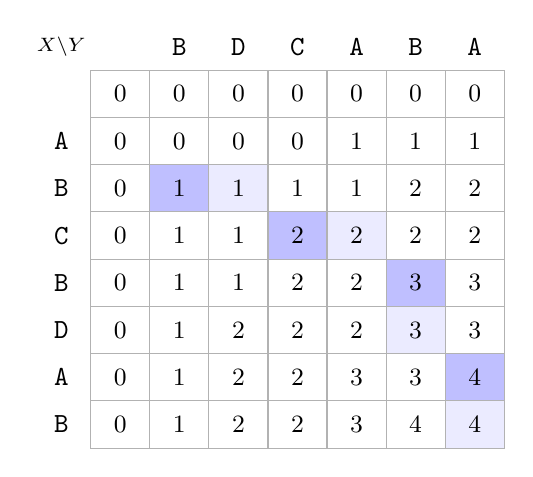
\begin{tikzpicture}[x=0.75cm, y=0.6cm, font=\small,
  cell/.style={draw, gray!60, text=black, minimum width=0.75cm, minimum height=0.6cm}]
  \node[font=\scriptsize] at (-1,1) {$X\backslash Y$};
  \node[font=\ttfamily] at (1,1) {B};
  \node[font=\ttfamily] at (2,1) {D};
  \node[font=\ttfamily] at (3,1) {C};
  \node[font=\ttfamily] at (4,1) {A};
  \node[font=\ttfamily] at (5,1) {B};
  \node[font=\ttfamily] at (6,1) {A};
  \node[font=\ttfamily] at (-1,-1) {A};
  \node[font=\ttfamily] at (-1,-2) {B};
  \node[font=\ttfamily] at (-1,-3) {C};
  \node[font=\ttfamily] at (-1,-4) {B};
  \node[font=\ttfamily] at (-1,-5) {D};
  \node[font=\ttfamily] at (-1,-6) {A};
  \node[font=\ttfamily] at (-1,-7) {B};
  \node[cell,] at (0,0) {0};
  \node[cell,] at (1,0) {0};
  \node[cell,] at (2,0) {0};
  \node[cell,] at (3,0) {0};
  \node[cell,] at (4,0) {0};
  \node[cell,] at (5,0) {0};
  \node[cell,] at (6,0) {0};
  \node[cell,] at (0,-1) {0};
  \node[cell,] at (1,-1) {0};
  \node[cell,] at (2,-1) {0};
  \node[cell,] at (3,-1) {0};
  \node[cell,] at (4,-1) {1};
  \node[cell,] at (5,-1) {1};
  \node[cell,] at (6,-1) {1};
  \node[cell,] at (0,-2) {0};
  \node[cell,fill=blue!25] at (1,-2) {1};
  \node[cell,fill=blue!8] at (2,-2) {1};
  \node[cell,] at (3,-2) {1};
  \node[cell,] at (4,-2) {1};
  \node[cell,] at (5,-2) {2};
  \node[cell,] at (6,-2) {2};
  \node[cell,] at (0,-3) {0};
  \node[cell,] at (1,-3) {1};
  \node[cell,] at (2,-3) {1};
  \node[cell,fill=blue!25] at (3,-3) {2};
  \node[cell,fill=blue!8] at (4,-3) {2};
  \node[cell,] at (5,-3) {2};
  \node[cell,] at (6,-3) {2};
  \node[cell,] at (0,-4) {0};
  \node[cell,] at (1,-4) {1};
  \node[cell,] at (2,-4) {1};
  \node[cell,] at (3,-4) {2};
  \node[cell,] at (4,-4) {2};
  \node[cell,fill=blue!25] at (5,-4) {3};
  \node[cell,] at (6,-4) {3};
  \node[cell,] at (0,-5) {0};
  \node[cell,] at (1,-5) {1};
  \node[cell,] at (2,-5) {2};
  \node[cell,] at (3,-5) {2};
  \node[cell,] at (4,-5) {2};
  \node[cell,fill=blue!8] at (5,-5) {3};
  \node[cell,] at (6,-5) {3};
  \node[cell,] at (0,-6) {0};
  \node[cell,] at (1,-6) {1};
  \node[cell,] at (2,-6) {2};
  \node[cell,] at (3,-6) {2};
  \node[cell,] at (4,-6) {3};
  \node[cell,] at (5,-6) {3};
  \node[cell,fill=blue!25] at (6,-6) {4};
  \node[cell,] at (0,-7) {0};
  \node[cell,] at (1,-7) {1};
  \node[cell,] at (2,-7) {2};
  \node[cell,] at (3,-7) {2};
  \node[cell,] at (4,-7) {3};
  \node[cell,] at (5,-7) {4};
  \node[cell,fill=blue!8] at (6,-7) {4};
\end{tikzpicture}
\caption{The LCS table $C[i][j]$ for $X=\texttt{ABCBDAB}$ and
$Y=\texttt{BDCABA}$. The traceback from the bottom-right corner is shaded;
dark cells are matches ($x_i=y_j$, move diagonally), which spell the LCS
\texttt{BCBA}.}
\end{figure}

\section{Edit distance}
The edit distance between $X$ and $Y$ is the minimum number of insertions, deletions, and substitutions turning $X$ into $Y$.
Let $D[i][j]$ = edit distance between $X[1..i]$ and $Y[1..j]$. Consider the last column of an optimal alignment:
\[
D[i][0]=i,\quad D[0][j]=j,\quad
D[i][j]=\min\begin{cases}
D[i-1][j]+1 & \text{delete }x_i,\\
D[i][j-1]+1 & \text{insert }y_j,\\
D[i-1][j-1]+[x_i\ne y_j] & \text{match/substitute.}
\end{cases}
\]
$\Theta(mn)$ time. (General costs, e.g.\ gap penalties in sequence alignment, work the same way.)
\begin{example}
$\texttt{kitten}\to\texttt{sitting}$ has distance 3: substitute k/s, substitute e/i, insert g.
\end{example}

\section{Longest increasing subsequence (LIS)}
Given $A[1..n]$, find the longest strictly increasing subsequence.
Let $L[i]$ be the length of the longest increasing subsequence \emph{ending at} $i$:
\[
L[i]=1+\max\{L[j]: j<i,\ A[j]<A[i]\}\quad(\max\emptyset=0).
\]
The answer is $\max_iL[i]$. Time $\Theta(n^2)$.

\paragraph{$\bigO(n\log n)$ improvement.} Maintain $T[k]$ = the smallest possible last element of an increasing subsequence
of length $k$ seen so far. $T$ is strictly increasing, so for each $A[i]$ binary search for the first $T[k]\ge A[i]$ and set
$T[k]=A[i]$ (or append if none). The final length of $T$ is the LIS length.

(Alternatively: LIS of $A$ $=$ LCS of $A$ and $\mathrm{sort}(A)$ with duplicates removed.)

\section{Matrix-chain multiplication}
Multiplying a $p\times q$ matrix by a $q\times r$ matrix costs $pqr$ scalar multiplications. Given $A_1\cdots A_n$ where $A_i$ is
$d_{i-1}\times d_i$, choose a parenthesization minimizing total cost. (Example: dimensions $10\times100$, $100\times5$, $5\times50$;
$(A_1A_2)A_3$ costs $5000+2500=7500$ while $A_1(A_2A_3)$ costs $25000+50000=75000$.)
The number of parenthesizations is the Catalan number $\Omega(4^n/n^{3/2})$, so brute force is hopeless.

Let $m[i][j]$ = min cost to compute $A_i\cdots A_j$. The last multiplication splits at some $k$:
\[
m[i][i]=0,\qquad m[i][j]=\min_{i\le k<j}\bigl(m[i][k]+m[k+1][j]+d_{i-1}d_kd_j\bigr).
\]
\begin{lstlisting}[style=pseudo]
for i = 1 to n do m[i][i] = 0
for len = 2 to n do                    // increasing interval length
    for i = 1 to n - len + 1 do
        j = i + len - 1; m[i][j] = $\infty$
        for k = i to j - 1 do
            c = m[i][k] + m[k+1][j] + $d_{i-1} d_k d_j$
            if c < m[i][j] then m[i][j] = c; s[i][j] = k
\end{lstlisting}
$\Theta(n^2)$ subproblems, $\bigO(n)$ each: $\Theta(n^3)$ time, $\Theta(n^2)$ space. This is the template for
\textbf{interval DP}: subproblems are contiguous ranges, evaluated by increasing length.

\begin{figure}[H]
\centering
\begin{tikzpicture}[x=0.7cm, y=0.7cm, font=\scriptsize, >=Stealth]
  \foreach \i in {1,...,5} \foreach \j in {\i,...,5} {
    \pgfmathtruncatemacro{\len}{\j-\i+1}
    \pgfmathsetmacro{\shade}{8+14*(\len-1)}
    \fill[blue!\shade] (\j-1,-\i) rectangle (\j,-\i+1);
    \draw (\j-1,-\i) rectangle (\j,-\i+1);
    \node at (\j-0.5,-\i+0.5) {\len};
  }
  \foreach \k in {1,...,5} {\node at (\k-0.5,1.3) {$j{=}\k$}; \node[anchor=east] at (-0.1,-\k+0.5) {$i{=}\k$};}
  \fill[red!30] (4,-1) rectangle (5,0); \draw[thick, red!70!black] (4,-1) rectangle (5,0);
  \node at (4.5,-0.5) {5};
  \draw[red!70!black, very thick, densely dashed] (0.05,-0.95) rectangle (3.95,-0.05);
  \draw[red!70!black, very thick, densely dashed] (4.05,-4.95) rectangle (4.95,-1.05);
  \node[anchor=west, align=left] at (5.5,-2) {$m[i][j]$ uses the row to its left\\and the column below it, i.e.\\only shorter intervals; fill\\diagonal by diagonal\\(numbers = length).};
\end{tikzpicture}
\caption{Evaluation order for interval DP with $n=5$: diagonals in order of
increasing length; the answer $m[1][n]$ is the top-right cell.}
\end{figure}

\section{Optimal binary search trees}
Keys $k_1<\dots<k_n$ with search probabilities $p_1,\dots,p_n$. Build a BST minimizing expected search cost
$\sum_i p_i(\mathrm{depth}(k_i)+1)$. (A balanced tree is not optimal when probabilities are skewed; greedy ``most likely key at
the root'' also fails.)

Let $e[i][j]$ be the minimum cost for keys $k_i..k_j$, and $w(i,j)=\sum_{t=i}^jp_t$. If $k_r$ is the root, every key in the subtree
moves one level deeper, adding $w(i,j)$:
\[
e[i][i-1]=0,\qquad e[i][j]=\min_{i\le r\le j}\bigl(e[i][r-1]+e[r+1][j]\bigr)+w(i,j).
\]
Same structure as matrix-chain: $\Theta(n^3)$ (Knuth's observation that the optimal root is monotone reduces this to $\Theta(n^2)$).
CLRS's version also includes probabilities $q_i$ for unsuccessful searches (dummy leaves); the recurrence is the same with $w$ adjusted.

\section{Top-down memoization}
Instead of ordering the loops, write the recursion directly and cache results:
\begin{lstlisting}[style=pseudo]
memo = empty table
LCS(i, j):
    if i == 0 or j == 0 then return 0
    if memo[i][j] defined then return memo[i][j]
    if $x_i = y_j$ then r = LCS(i-1, j-1) + 1
    else r = max(LCS(i-1, j), LCS(i, j-1))
    memo[i][j] = r; return r
\end{lstlisting}
Same asymptotics; only reachable subproblems are computed, at the cost of recursion overhead.

\section{Pitfalls}
\begin{itemize}
  \item State the meaning of every table entry in words; most wrong DPs come from vague subproblem definitions.
  \item ``Ending at $i$'' vs.\ ``using a prefix up to $i$'' are different subproblems (LIS uses the former, knapsack the latter).
  \item Check that the evaluation order respects dependencies (interval DP: by length, not by $i$).
  \item Count work per subproblem: matrix-chain is $\Theta(n^3)$, not $\Theta(n^2)$.
\end{itemize}

\section*{Summary}
\begin{center}
\begin{tabular}{lll}
\toprule
Problem & Subproblem & Time \\
\midrule
Weighted interval scheduling & best on intervals $1..j$ & $\Theta(n\log n)$ \\
0/1 knapsack & items $1..i$, capacity $w$ & $\Theta(nW)$ (pseudo-poly) \\
LCS / edit distance & prefixes $X[1..i],Y[1..j]$ & $\Theta(mn)$ \\
LIS & ending at $i$ & $\Theta(n^2)$ or $\Theta(n\log n)$ \\
Matrix chain / optimal BST & interval $[i,j]$ & $\Theta(n^3)$ \\
\bottomrule
\end{tabular}
\end{center}
